\section{METODOLOGI}

% Ubah paragraf-paragraf berikut sesuai dengan isi dari metodologi
Metode yang kami gunakan adalah \lipsum[10]

% Contoh input gambar dengan format *.jpg
\begin{figure} [ht] \centering
  % Nama dari file gambar yang diinputkan
  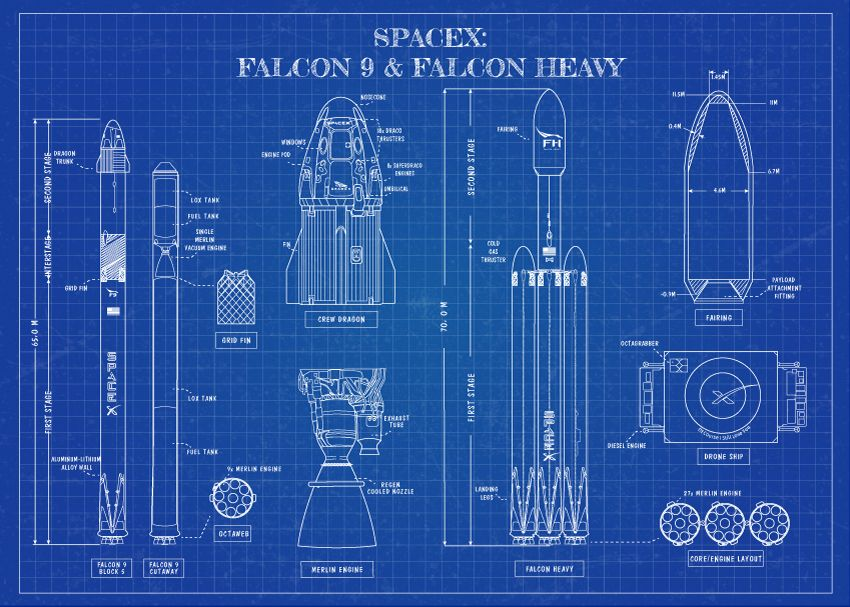
\includegraphics[scale=0.45]{gambar/blueprint.jpg}
  % Keterangan gambar yang diinputkan
  \caption{\emph{Blueprint} roket yang akan diuji coba}
  % Label referensi dari gambar yang diinputkan
  \label{fig:blueprint}
\end{figure}

% Contoh penggunaan referensi dari gambar yang diinputkan
Pada \emph{blueprint} yang tertera di \ref{fig:blueprint}. \lipsum[11]

\lipsum[12]